\subsection{复圆函数；双曲函数}

欧拉公式 (25)（III, p.~99）与 \(e^z\) （对每个复数 \(z\) 而言）的定义，使我们可以向 \(\mathbf{C}\) 延拓函数 \(\cos x\) 与 \(\sin x\) ——它们定义在 \(\mathbf{R}\) 上——，只需对一切 \(z \in \mathbf{C}\) 令

\[
\cos z = \frac {1}{2} \left(e ^ {i z} + e ^ {- i z}\right), \quad \sin z = \frac {1}{2 i} \left(e ^ {i z} - e ^ {- i z}\right)\tag{32}
\]

（cf.~III, p.~119, exerc. 19）。

这些函数是以 \(2\pi\) 为最小周期的周期函数；即有 \(\cos(z + \pi/2) = -\sin z\) ，\(\sin(z + \pi/2) = \cos z\) ；还可以验证恒等式

\[
\begin{array}{c} \cos^ {2} z + \sin^ {2} z = 1 \\ \cos (z + z ^ {\prime}) = \cos z \cos z ^ {\prime} - \sin z \sin z ^ {\prime} \\ \sin (z + z ^ {\prime}) = \sin z \cos z ^ {\prime} + \cos z \sin z ^ {\prime}. \end{array}
\]

更一般地，实变量圆函数之间的每个代数恒等式当这些变量取任意复值时仍然成立（III, p.~119, exerc. 18）。

令 \(\tan z = \sin z/\cos z\) （若 \(z \neq (2k + 1)\pi/2\) ），令 \(\cot z = \cos z/\sin z\) （若 \(z \neq k\pi\) ）；它们是以 \(\pi\) 为最小周期的周期函数。

公式 (27)（III, p.~99）表明 \(\cos z\) 与 \(\sin z\) 在 \(\mathbf{C}\) 上可导，并且

\[
\mathrm{D} (\cos z) = - \sin z, \quad \mathrm{D} (\sin z) = \cos z.
\]

对 \(z = ix\) （x 为实数），公式 (32) 给出

\[
\cos i x = \frac {1}{2} \left(e ^ {x} + e ^ {- x}\right), \quad \sin i x = \frac {i}{2} \left(e ^ {x} - e ^ {- x}\right).
\]

对这样引入的实函数，采用专门的记号是方便的；我们令

\[
\left\{ \begin{array}{l l} \cosh x = \frac {1}{2} \left(e ^ {x} + e ^ {- x}\right) & \text {(hyperbolic cosine of x)} \\ \sinh x = \frac {i}{2} \left(e ^ {x} - e ^ {- x}\right) & \text {(hyperbolic sine of x)} \\ \tanh x = \frac {\sinh x}{\cosh x} = \frac {e ^ {x} - e ^ {- x}}{e ^ {x} + e ^ {- x}} & \text {(hyperbolic tangent of x)} \end{array} \right.\tag{33}
\]

于是，对每个实数 \(x\)

\[
\cos i x = \cosh x, \quad \sin i x = i \sinh x.\tag{34}
\]

由若干复数 \(z_{k}\) （ \(1 \leqslant k \leqslant n\) ）的圆函数之间的每个恒等式，把 \(z_{k}\) 换成 \(ix_{k}\) （ \(x_{k}\) 为实数，\(1 \leqslant k \leqslant n\) ）并利用公式 (34)，就可以得到双曲函数的一个恒等式；例如有

\[
\begin{array}{c} \cosh^ {2} x - \sinh^ {2} x = 1 \\ \cosh (x + x ^ {\prime}) = \cosh x \cosh x ^ {\prime} + \sinh x \sinh x ^ {\prime} \\ \sinh (x + x ^ {\prime}) = \sinh x \cosh x ^ {\prime} - \cosh x \sinh x ^ {\prime}. \end{array}
\]

双曲函数使我们可以表出 \(\cos z\) 与 \(\sin z\) 当 \(z = x + iy\) 时的实部与虚部，因为

\[
\begin{array}{l} \cos (x + i y) = \cos x \cos i y - \sin x \sin i y = \cos x \cosh y - i \sin x \sinh y \\ \sin (x + i y) = \sin x \cos i y + \cos x \sin i y = \sin x \cosh y + i \cos x \sinh y. \end{array}
\]

最后，有

\[
\mathrm{D} (\cosh x) = \sinh x, \mathrm{D} (\sinh x) = \cosh x, \mathrm{D} (\tanh x) = 1 - \tanh ^ {2} x = \frac {1}{\cosh^ {2} x}.
\]

由于对一切 x 有 \(\cosh x > 0\) ，由此推出 \(\sinh x\) 在 R 上严格递增；又 \(\sinh 0 = 0\) ，故 \(\sinh x\) 与 x 同号。于是 \(\cosh x\) 在 \(x \leqslant 0\) 时严格递减，在 \(x \geqslant 0\) 时严格递增；最后，\(\tanh x\) 在 R 上严格递增。此外

\[
\begin{array}{l} \lim _ {x \to - \infty} \sinh x = - \infty , \quad \lim _ {x \to + \infty} \sinh x = + \infty \\ \lim _ {x \to - \infty} \cosh x = \lim _ {x \to + \infty} \cosh x = + \infty \\ \lim _ {x \to - \infty} \tanh x = - 1, \quad \lim _ {x \to + \infty} \tanh x = + 1 \quad (\text {   fig.   8   and   9   }). \end{array}
\]

有时以 \(\operatorname{Arg}\sinh x\) 表示 \(\sinh x\) 的反函数，它是 \(\mathbf{R}\) 到 \(\mathbf{R}\) 上的严格递增映射；这个函数也可以用对数表示，因为由关系式 \(x = \sinh y = \frac{1}{2}(e^y - e^{-y})\) 推出 \(e^{2y} - 2xe^y - 1 = 0\) ，而由于 \(e^y > 0\) ，有 \(e^y = x + \sqrt{x^2 + 1}\) ，也就是说

\[
\operatorname{Arg} \sinh x = \log (x + \sqrt {x ^ {2} + 1}).
\]

类似地，我们把 \(\operatorname{Arg}\cosh x\) 记为 \(\cosh x\) 在 \([0, +\infty[\) 上的限制的反函数；这个映射是 \([1, +\infty[\) 到 \([0, +\infty[\) 上的严格递增映射；与上面一样可以证明

\[
\operatorname{Arg} \cosh x = \log (x + \sqrt {x ^ {2} - 1}).
\]

\pandocbounded{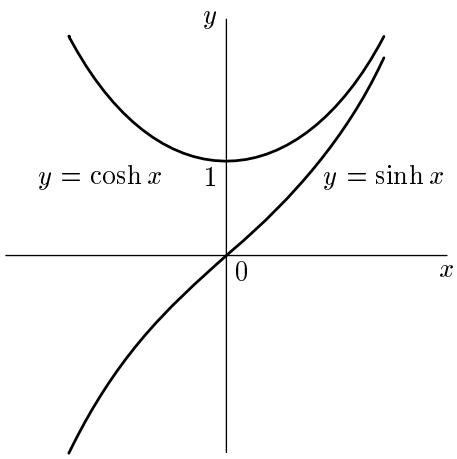
\includegraphics[keepaspectratio]{images/part001_d9e35212.jpg}}\\
图 8

\pandocbounded{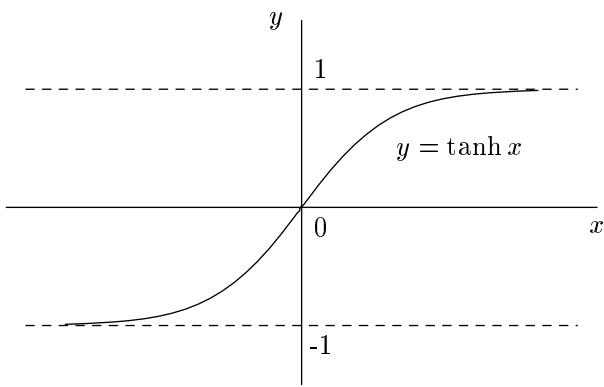
\includegraphics[keepaspectratio]{images/part001_f5896466.jpg}}\\
图 9

最后，我们以 \(\operatorname{Arg}\tanh x\) 表示 \(\tanh x\) 的反函数，它是 \(] - 1, +1[\) 到 \(\mathbf{R}\) 上的严格递增映射；此外有

\[
\operatorname{Arg} \tanh x = \frac {1}{2} \log \frac {1 + x}{1 - x}.
\]

注。对复数 \(z\) ，有时写

\[
\begin{array}{l} \cosh z = \frac {1}{2} (e ^ {z} + e ^ {- z}) = \cos i z \\ \sinh z = \frac {1}{2} (e ^ {z} - e ^ {- z}) = - i \sin i z. \end{array}
\]

这些函数就这样把定义在 R 上的双曲函数延拓到了 C。

